\documentclass{article}
\usepackage[utf8]{inputenc}
\usepackage[T1]{fontenc}
\usepackage[francais]{babel}
\usepackage{amsmath}
\usepackage{graphicx}
\usepackage{color}
\usepackage{framed}
\usepackage{marvosym}
\usepackage{pifont}
\usepackage[top=2cm, bottom=2cm, left=2cm, right=2cm]{geometry}
\usepackage{pdfpages} 
\usepackage{listings}
\usepackage{graphicx}
\usepackage{hyperref}
\usepackage{amsthm}
\usepackage{amssymb}
\usepackage{mathrsfs}
\usepackage{verbatim}
\usepackage{moreverb}
\usepackage{titletoc}


\definecolor{oxf}{RGB}{0, 33, 71}
\definecolor{or}{RGB}{239, 155, 15}
\definecolor{vert}{RGB}{135,167,103}
\definecolor{rouge}{RGB}{181,39,39}
\definecolor{violet}{RGB}{64,9,90}


\newcommand{\Div}[2]{
\definecolor{shadecolor}{gray}{0.9}
\begin{leftbar}
\begin{shaded}
\textbf{#1}\\
\textit{#2}
\end{shaded}
\end{leftbar}
\bigskip
}


\newcommand{\Def}[2]{
\definecolor{shadecolor}{RGB}{239, 155, 15}
\begin{leftbar}
\begin{shaded}
 \textcolor{white}{\textbf{\textit{\ding{247} Définition:}} \textbf{\textit{#1}}}
\end{shaded}
#2
\end{leftbar}
\bigskip
}

\newcommand{\Th}[2]{
\definecolor{shadecolor}{RGB}{0, 33, 71}
\begin{leftbar}
\begin{shaded}
 \textcolor{white}{\textbf{\textit{\ding{49} Théorème:}} \textbf{\textit{#1}}}
\end{shaded}
#2
\end{leftbar}
\bigskip
}

\newcommand{\Lem}[2]{
\definecolor{shadecolor}{RGB}{0, 33, 71}
\begin{leftbar}
\begin{shaded}
 \textcolor{white}{\textbf{\textit{\ding{49} Lemme:}} \textbf{\textit{#1}}}
\end{shaded}
#2
\end{leftbar}
\bigskip
}

\newcommand{\Cor}[2]{
\definecolor{shadecolor}{RGB}{0, 33, 71}
\begin{leftbar}
\begin{shaded}
 \textcolor{white}{\textbf{\textit{\ding{49} Corollaire:}} \textbf{\textit{#1}}}
\end{shaded}
#2
\end{leftbar}
\bigskip
}

\newcommand{\Exe}[2]{
\definecolor{shadecolor}{RGB}{181,39,39}
\begin{leftbar}
\begin{shaded}
 \textcolor{white}{\textbf{\textit{\Coffeecup Exercice:}} \textbf{\textit{#1}}}
\end{shaded}
#2
\end{leftbar}
\bigskip
}


\newcommand{\Rem}[2]{
\definecolor{shadecolor}{RGB}{135,167,103}
\begin{leftbar}
\begin{shaded}
 \textcolor{white}{\textbf{\textit{\Info  Remarque:}} \textbf{\textit{#1}}}
\end{shaded}
#2
\end{leftbar}
\bigskip
}

\newcommand{\Prop}[2]{
\definecolor{shadecolor}{RGB}{135,167,103}
\begin{leftbar}
\begin{shaded}
 \textcolor{white}{\textbf{\textit{\Info  Propriété:}} \textbf{\textit{#1}}}
\end{shaded}
#2
\end{leftbar}
\bigskip
}

%Macros pour modifier la table des matières
\hypersetup{colorlinks=true, urlcolor=bleu, linkcolor=black}
\usepackage{hyperref}

\titlecontents{chapter}[20pt]% 103
   {\addvspace{1pc}\normalfont\sffamily\bfseries\large} 
            {\contentslabel[\thecontentslabel]{20pt}}{}{\hfill\contentspage}[] 
\titlecontents{subsection}[40pt]% 
   {\addvspace{0.6pc}\normalfont\sffamily} 
            {\contentslabel[\thecontentslabel]{25pt}}{}{\dotfill\contentspage}[] 
\titlecontents{subsubsubsection}[60pt]% 
   {\addvspace{0.3pc}\normalfont\sffamily} 
            {\contentslabel[\thecontentslabel]{25pt}}{}{\dotfill\contentspage}[]                            
\titlecontents*{subsubsubsubsection}[60pt]% 
   {\filright\normalfont\sffamily\footnotesize}{}{}{}[~{–}\ ][] 
\setcounter{tocdepth}{3}

\makeatletter\@addtoreset{subsection}{part}
\makeatother



\newtheorem*{Dem}{Démonstration}


\begin{document}
\tableofcontents
\newpage

\part{Cours}
\section{\textit{Gestionnaires de paquets}}
\subsection{Dans la famille Debian}
\subsubsection{Installation des paquets}

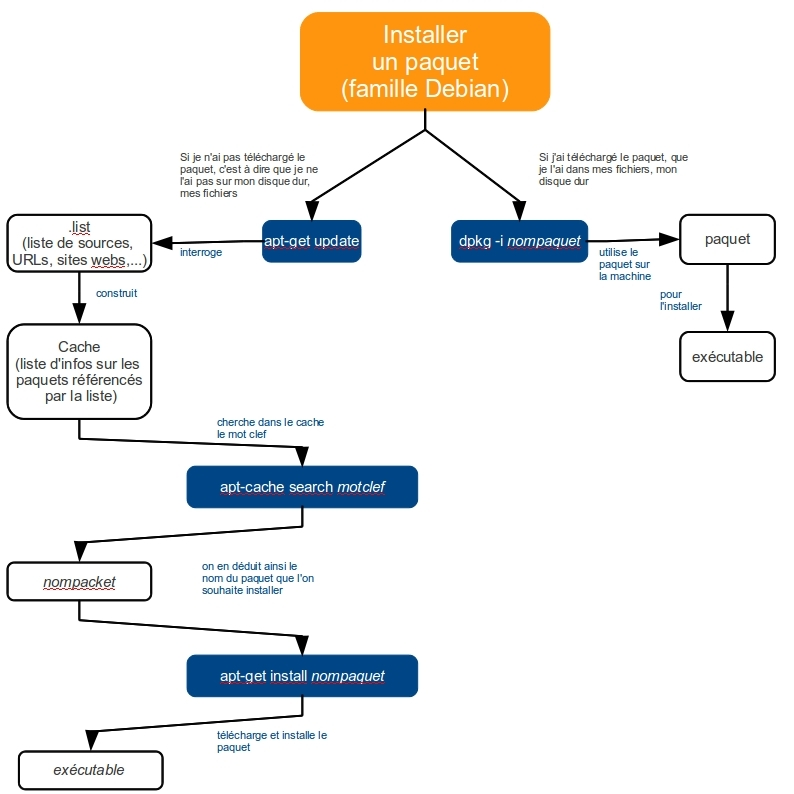
\includegraphics[scale=4]{gestDeb.jpg}

On peut aussi simuler l'installation, dans ce cas, on utilise: \textbf{apt-get install -s \textit{nompaquet}}.\\

\subsubsection{Suppression de paquets}

On peut aussi vouloir faire l'opération inverse de l'installation: la suppression, dans ce cas, on utilise: 
\textbf{apt-get remove \textit{nompaquet}} ou \textbf{apt-get remove --purge \textit{nompaquet}} si l'on veut en plus supprimer
les fichiers de configuration. 

\Rem{}{Garder les fichiers de configuration permettrait de disposer de celle-ci lors d'une installation ultérieure et donc de ne pas avoir la
configuration par défault.}

\subsubsection{Reconfiguration des paquets}
Pour reconfigurer les paquets avec la configuration par défault (i.e. celle à l'installation), on utilise la commande: \textbf{dpkg --reconfigure \textit{nompaquet}}.

\subsubsection{Mise à jour des paquets installés}
On utilise: \textbf{apt-get upgrade} ou \textbf{apt-get dist-upgrade} si l'on veut faire attention aux dépendances lors de la mise à jour. L'option \textbf{-u} permet de connaître
les paquets qui vont être mis à jour.

\subsubsection{Informations sur un paquet}

\textbf{apt-cache show \textit{nompaquet}} nous permet d'obtenir des détails sur le paquet.\\

\textbf{apt-cache depends \textit{nompaquet}} nous donne les dépendances du paquet.\\

\subsection{Dans la famille RedHat}
\subsubsection{L'outil rpm}
Il n'existe pas vraiment d'outil de gestion avancée des paquets. On utilise pour gérer les paquets la commande rpm (RedHat Package Manager) \\
\begin{description}
	\item[Installation :]rpm -ivh <paquet.rpm>
	\item[Mise à jour : ] rpm -Uvh <paquet.rpm>
	\item[Forçage install :]rpm -o --nodeps --force <paquet.rpm>
	\item[Désinstaller :] rpm -e <logiciel>
	\item[Dépendance d'un paquet installé :] rpm -qi <nom paquetage>
	\item[De même mais non installé :] rpm -qip <nom paquetage>
	\item[Liste des logiciels installés :] rpm -qa
\end{description}

\subsubsection{L'outil yum}
Pour combler le manque de rpm concernant les dépendances, un outil a été développé : yum. Il permet de définir plusieurs serveurs sur lesquels aller chercher les paquets ainsi que leurs dépendances.

\paragraph{Configurer yum : \\}
Ils s'agit en fait de créer des fichier \textit{file.repo} dans le dossier \textit{/etc/yum.repos.d}. 

\paragraph{Utilisation de yum : \\}
\begin{description}
	\item[Mise à jour système :] yum update
	\item[Mise à jour séléctive :] yum --exclude=<nom paquet> update
	\item[Exclure dépôt temporairement :] yum --disablerepo=<nom dépot> update
	\item[Réinclude ce dépôt :] yum --enablerepo=... update
	\item[Rechercher un paquet :] yum list <nom paquet>
	\item[Installer un paquet :] yum install <nom paquet>
	\item[Supprimer un paquet :]yum remove <nom paquet>
\end{description}

\section{Le shell}
Ce langage ne nécessite pas de compilation, il est directement exécutable, interprétable. On distingue deux familles : \begin{itemize}
	\item csh (qui compte tcsh par exemple)
	\item sh (bash par exemple)
\end{itemize}

Voir TD

\newpage
\part{TD}
\section{Adimnistration système}
Contenu des différents fichiers à la racine : 
\begin{description}
	\item[/bin :] Commandes essentielles communes à tous les utilisateurs
	\item[/boot :] Fichier de démarrage système
	\item[/dev :] Point d'entrée des périphériques
	\item[/etc :] Fichiers de configuration
	\item[/home :] Répertoires personnels
	\item[/root :] Répertoire de l'administrateur
	\item[/usr :] Hiérarchie secondaire, applications, bibliothèques partagées
	\item[/var :] Logs du système, fichiers traces.
	\item[/proc :] Système de fichier virtuel, informations en temps réel
\end{description}

\bigskip
Liste de commandes utiles et oubliées :
\begin{description}
	\item[pwd :]afficher le répertoire courant
	\item[file :] afficher le type de contenu du fichier
	\item[locate :] localiser un fichier sur le disque
	\item[passwd LOGIN :]changer le mot de passe
	\item[adduser / deluser / usermode :] utilisable par root, permet d'ajouter ou de supprimer un utilisateur, ou de changer les propriétés d'un compte
	\item[ps / ps aux / pstree :] affiche processus utilisateur, ou tous les processus du système, ou sous forme d'arborescence
	\item[top :] outil semi-graphique présentant un grand nombre d'info sur les processus
	\item[fdisk -l :] voir toutes les partitions
	\item[mount -t SYSTFICHIER PERIPHERIQUE REPERTOIRE :] monter un périphérique (en général dans /media)
\end{description}

Référencement de tous les utilisateurs dans les fichiers \textit{/etc/passwd} ou \textit{/etc/shadow}.

\paragraph{Partitions :\\}
Il existe 3 types de partition : \begin{itemize}
	\item Partition principale : 4 au maximum, pour tout type de système de fichiers
	\item Partition étendue : ne contient que des partitions logiques, et elle n'existe qu'avec une partition principale
	\item Partition logique : contenue dans une partition étendue, avec un système de fichier, nombre infini.
\end{itemize}

On compte aussi une partition "swap", utilié pour décharger la mémoire vive, et le MBR (Master Boot Recorder), où est installé un chargeur (Grub)
\section{Shell bash}



\end{document}
